\documentclass{beamer}

\usepackage[utf8]{inputenc}
\usepackage{xcolor}
\usepackage{enumerate}
\usepackage{mathtools}
\usepackage{multicol}
\usepackage{bbm}
\usepackage{latexsym, amssymb, amscd, amsthm, amsxtra, amsmath, amsthm}
\usepackage{graphics, graphicx, color}
\usepackage{natbib}
\usepackage{ifpdf}
\usepackage[format=hang,indention=-1cm,small]{caption}
\usepackage[caption=false]{subfig}
\usepackage{multirow}
\usepackage{kotex}
\usepackage{hyperref}
\DeclareGraphicsExtensions{.pdf,.png,.jpg}
\usetheme[]{Madrid}

%Information to be included in the title page:
\title[VI based Recommender systems]{Recommender systems based on variational inference}
\author[Team 10]{Kunwoong Kim \and Dongwuk Kim \and Minwoo Kim }
\institute[]{Team 10 \\ Graduate Student, Seoul National Univeristy, Department of Statistics}
\date[\today]{\today}
 
\begin{document}

% THEOREMS -------------------------------------------------------
\newtheorem{thm}{Theorem}
\newtheorem{cor}[thm]{Corollary}
\newtheorem{lem}[thm]{Lemma}
\newtheorem{prop}[thm]{Proposition}
\theoremstyle{definition}
\newtheorem{defn}{Definition}
\newtheorem*{defn*}{Definition}
\theoremstyle{remark}
\newtheorem{remark}{Remark}
%\newtheorem{example}{Example}
\newtheorem{Rule}{Rule}
\newtheorem{Assumption}{Assumption}

%\numberwithin{equation}{chapter}

% MATH -----------------------------------------------------------
\newcommand{\norm}[1]{\left\Vert#1\right\Vert}
\newcommand{\abs}[1]{\left\vert#1\right\vert}
\newcommand{\set}[1]{\left\{#1\right\}}
\newcommand{\Real}{\mathbb R}
\newcommand{\Nb}{\mathbb N}
\newcommand{\eps}{\varepsilon}
\newcommand{\To}{\longrightarrow}
\newcommand{\BX}{\mathbf{B}(X)}
\newcommand{\A}{\mathfrak{A}}
\newcommand{\Exp}{\mathrm{Exp}}
\newcommand{\Log}{\mathrm{Log}}
\newcommand{\vx}{\mathbf{x}}
\renewcommand{\thefootnote}{\fnsymbol{footnote}} 	
\def\argmin{\mathop{\rm argmin}}
\def\argmax{\mathop{\rm argmax}}
\def\Cov{\mbox{Cov}}
\def\Corr{\mbox{Corr}}
\def\Var{\mbox{Var}}
\def\ang{\mbox{Angle}}
\def\E{\mbox{E}}
\def\tr{\mbox{trace}}
\def\half{\frac{1}{2}}
\def\proj{\mbox{Proj}}
\def\diag{\mbox{diag}}
\def\rank{\mbox{rank}}
\def\symp{\mbox{Sym}^+}
\def\sym{\mbox{Sym}}
\def\SO{\mbox{SO}}
\def\O{\mbox{O}}
\def\GL{\mbox{GL}}
\def\asym{\mathfrak{so}}
\def\so{\mathfrak{so}}
\def\diagp{\mbox{Diag}^+}
\def\diag{\mbox{Diag}}
\def\matd{\mbox{matd}}
\def\vecd{\mbox{vecd}}
\def\To{\longrightarrow}
\def\Complex{\mathbb{C}}
\def\C{\mathbb{C}}

\def\av{\mathbf a}
\def\bv{\mathbf b}
\def\cv{\mathbf c}
\def\dv{\mathbf d}
\def\ev{\mathbf e}
\def\fv{\mathbf f}
\def\gv{\mathbf g}
\def\hv{\mathbf h}
\def\iv{\mathbf i}
\def\jv{\mathbf j}
\def\gv{\mathbf g}
\def\kv{\mathbf k}
\def\lv{\mathbf l}
\def\mv{\mathbf m}
\def\nv{\mathbf n}
\def\ov{\mathbf o}
\def\pv{\mathbf p}
\def\qv{\mathbf q}
\def\rv{\mathbf r}
\def\sv{\mathbf s}
\def\tv{\mathbf t}
\def\uv{\mathbf u}
\def\vv{\mathbf v}
\def\wv{\mathbf w}
\def\xv{\mathbf x}
\def\yv{\mathbf y}
\def\zv{\mathbf z}

\def\Av{\mathbf A}
\def\Bv{\mathbf B}
\def\Cv{\mathbf C}
\def\Dv{\mathbf D}
\def\Ev{\mathbf E}
\def\Fv{\mathbf F}
\def\Gv{\mathbf G}
\def\Hv{\mathbf H}
\def\Iv{\mathbf I}
\def\Jv{\mathbf J}
\def\Kv{\mathbf K}
\def\Lv{\mathbf L}
\def\Mv{\mathbf M}
\def\Nv{\mathbf N}
\def\Ov{\mathbf O}
\def\Pv{\mathbf P}
\def\Qv{\mathbf Q}
\def\Rv{\mathbf R}
\def\Sv{\mathbf S}
\def\Tv{\mathbf T}
\def\Uv{\mathbf U}
\def\Vv{\mathbf V}
\def\Wv{\mathbf W}
\def\Xv{\mathbf X}
\def\Yv{\mathbf Y}
\def\Zv{\mathbf Z}

\newcommand{\alphav}{\mbox{\boldmath{$\alpha$}}}
\newcommand{\betav}{\mbox{\boldmath{$\beta$}}}
\newcommand{\gammav}{\mbox{\boldmath{$\gamma$}}}
\newcommand{\deltav}{\mbox{\boldmath{$\delta$}}}
\newcommand{\epsilonv}{\mbox{\boldmath{$\epsilon$}}}
\newcommand{\zetav}{\mbox{\boldmath$\zeta$}}
\newcommand{\etav}{\mbox{\boldmath{$\eta$}}}
\newcommand{\iotav}{\mbox{\boldmath{$\iota$}}}
\newcommand{\kappav}{\mbox{\boldmath{$\kappa$}}}
\newcommand{\lambdav}{\mbox{\boldmath{$\lambda$}}}
\newcommand{\muv}{\mbox{\boldmath{$\mu$}}}
\newcommand{\nuv}{\mbox{\boldmath{$\nu$}}}
\newcommand{\xiv}{\mbox{\boldmath{$\xi$}}}
\newcommand{\omicronv}{\mbox{\boldmath{$\omicron$}}}
\newcommand{\piv}{\mbox{\boldmath{$\pi$}}}
\newcommand{\rhov}{\mbox{\boldmath{$\rho$}}}
\newcommand{\sigmav}{\mbox{\boldmath{$\sigma$}}}
\newcommand{\tauv}{\mbox{\boldmath{$\tau$}}}
\newcommand{\upsilonv}{\mbox{\boldmath{$\upsilon$}}}
\newcommand{\phiv}{\mbox{\boldmath{$\phi$}}}
\newcommand{\varphiv}{\mbox{\boldmath{$\varphi$}}}
\newcommand{\chiv}{\mbox{\boldmath{$\chi$}}}
\newcommand{\psiv}{\mbox{\boldmath{$\psi$}}}
\newcommand{\omegav}{\mbox{\boldmath{$\omega$}}}
\newcommand{\Sigmav}{\mbox{\boldmath{$\Sigma$}}}
\newcommand{\Lambdav}{\mbox{\boldmath{$\Lambda$}}}
\newcommand{\Deltav}{\mbox{\boldmath{$\Delta$}}}

\newcommand{\Ac}{\mathcal{A}}
\newcommand{\Bc}{\mathcal{B}}
\newcommand{\Cc}{\mathcal{C}}
\newcommand{\Dc}{\mathcal{D}}
\newcommand{\Ec}{\mathcal{E}}
\newcommand{\Fc}{\mathcal{F}}
\newcommand{\Gc}{\mathcal{G}}
\newcommand{\Hc}{\mathcal{H}}
\newcommand{\Ic}{\mathcal{I}}
\newcommand{\Jc}{\mathcal{J}}
\newcommand{\Kc}{\mathcal{K}}
\newcommand{\Lc}{\mathcal{L}}
\newcommand{\Mc}{\mathcal{M}}
\newcommand{\Nc}{\mathcal{N}}
\newcommand{\Oc}{\mathcal{O}}
\newcommand{\Pc}{\mathcal{P}}
\newcommand{\Qc}{\mathcal{Q}}
\newcommand{\Rc}{\mathcal{R}}
\newcommand{\Sc}{\mathcal{S}}
\newcommand{\Tc}{\mathcal{T}}
\newcommand{\Uc}{\mathcal{U}}
\newcommand{\Vc}{\mathcal{V}}
\newcommand{\Wc}{\mathcal{W}}
\newcommand{\Xc}{\mathcal{X}}
\newcommand{\Yc}{\mathcal{Y}}
\newcommand{\Zc}{\mathcal{Z}}
\newcommand{\J}{\sf J}
\newcommand{\mb}{\mbox}

% Slide begin
\begin{frame}
  \titlepage
\end{frame}

\AtBeginSection[]
{
  \begin{frame}
    \frametitle{Current Section}
    \tableofcontents[currentsection, hideothersubsections]
  \end{frame}
}

\section{Recommender system}
\begin{frame}{User ratings matrix}
	\begin{figure}
		\centering
		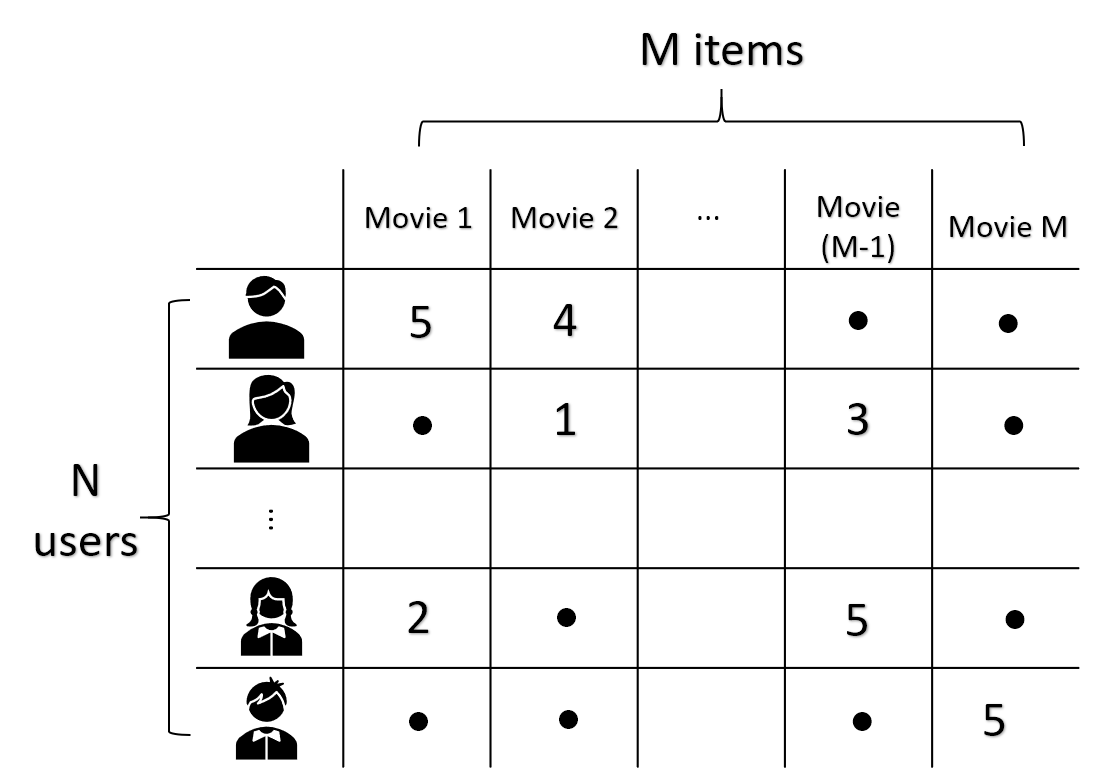
\includegraphics[width=0.7\linewidth]{fig/ppt-fig1}
		\caption{Example of user ratings}
		\label{fig:ppt-fig1}
	\end{figure}
\end{frame}

\begin{frame}{Matrix Factorization}
	\begin{figure}
		\centering
		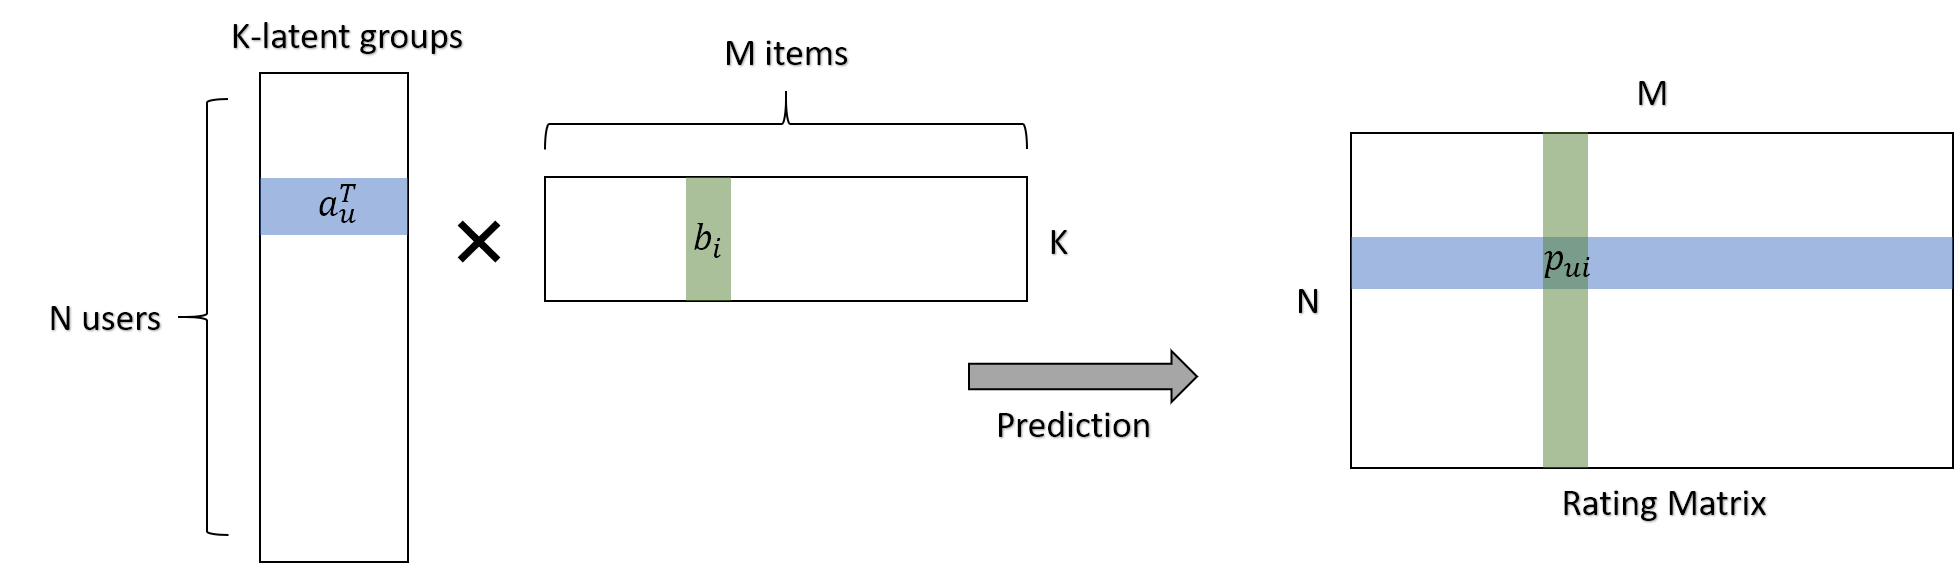
\includegraphics[width=0.9\linewidth]{fig/ppt-fig2}
		%\caption{Example of user ratings}
		\label{fig:ppt-fig2}
	\end{figure}
	\begin{itemize}
		\item $K \in \Nb$ latent factor: groups of users who share the same tastes.  
		\item $ \av_u \in \Real^{K} $: $\av_{u, k} = \Pr(\text{user } u \in \text{Group } K),$ so $ \sum_{k=1}^{K} \av_{u, k}  = 1$. 
		\item $ \bv_i \in \Real^{K} $: $\bv_{u, k} = \Pr(\text{users in the group } k \text{ like item } i).$
		\item $ \pv_{u, i} = \av_u^T\bv_i$ : estimated rating (up to scaling).
	\end{itemize}
\end{frame}

\begin{frame}{Example}
	\begin{figure}
		\centering
		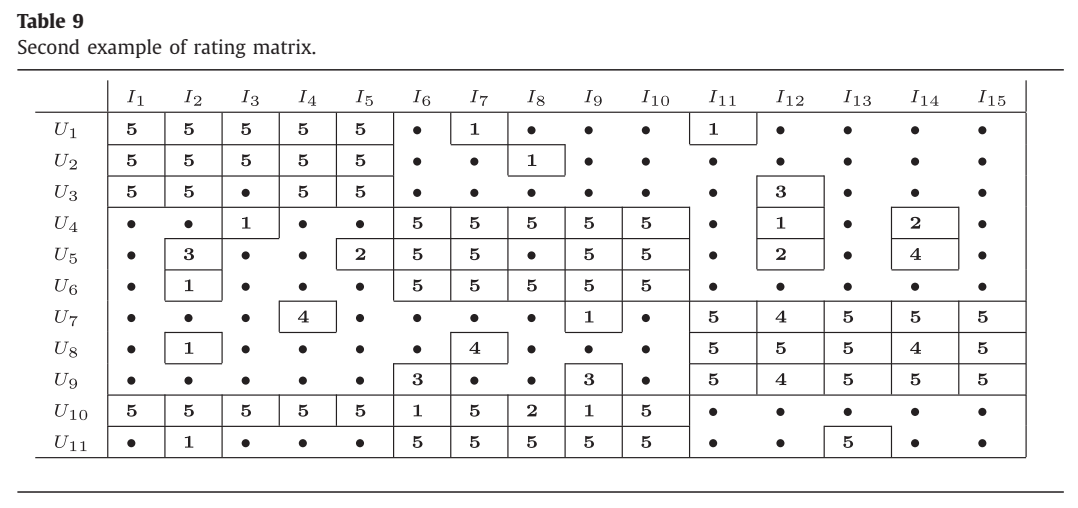
\includegraphics[width=0.9\linewidth]{fig/Table9}
		%\caption{Example of user ratings}
		\label{fig:table9}
	\end{figure}
\end{frame}

\begin{frame}{Example}
	\begin{figure}
		\centering
		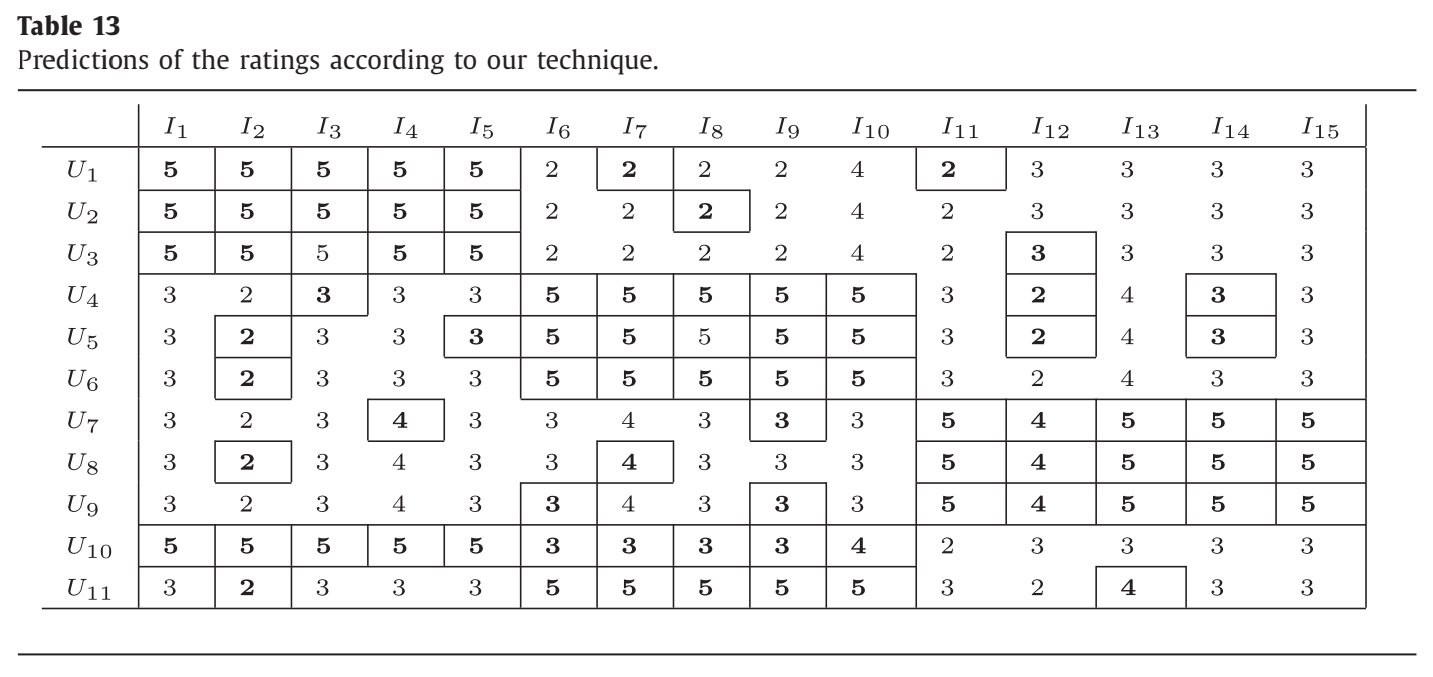
\includegraphics[width=0.9\linewidth]{fig/Table13}
		%\caption{Example of user ratings}
		\label{fig:table13}
	\end{figure}
	\begin{itemize}
		\item Make a prediction and recommend items to user.
	\end{itemize}
\end{frame}

\begin{frame}{Proposed method}
    \begin{itemize}
        \item Antonio Hernando et al., 
        \textcolor{blue}{A non negative matrix factorization for collaborative filtering recommender systems based on a Bayesian probabilistic model}, \textit{Knowledge-Based Systems}, volume 97, 2016, 188–202
        \item Adopt a latent graphical model for $\av_u, \bv_i$ and $ \pv_{u, i} $.
        \item Use variational inference to estimate a ratings matrix.
    \end{itemize}
\end{frame}

\begin{frame}{Structure of the presentation}
	\begin{enumerate}
        \item Understanding the model and algorithm.
        \item Evaluations of the model performance.
		\item Applications to various domain: Steam games, Book recommendation.
		\item Discussion.
	\end{enumerate}
\end{frame}

\section{Method}

\begin{frame}{Graphical model}
	\begin{figure}
		\centering
		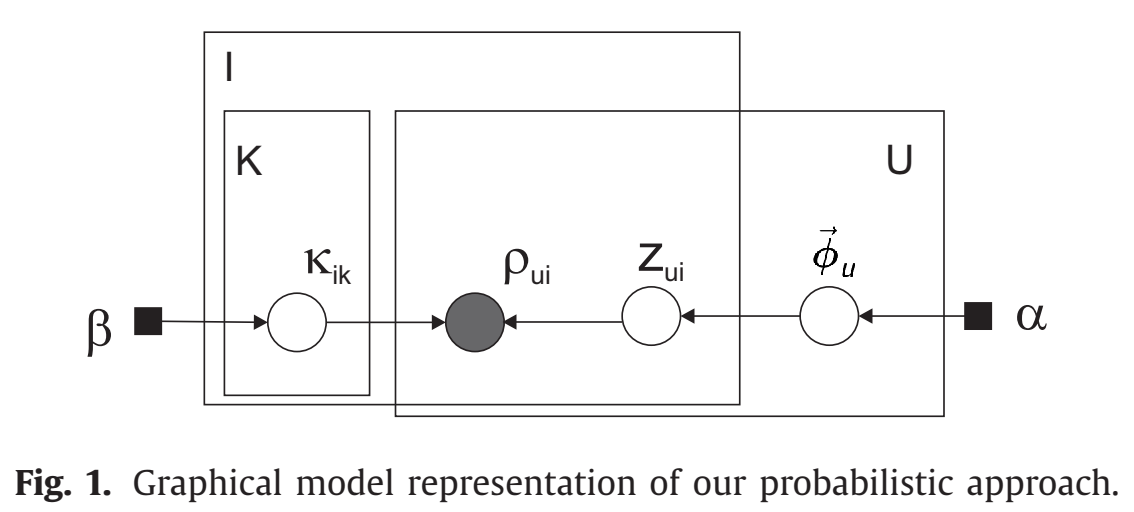
\includegraphics[width=0.7\linewidth]{fig/graphical}
		%\caption{Example of user ratings}
		\label{fig:table9}
	\end{figure}
    \begin{itemize}
        \item $ \vec{\phiv}_u \sim Dir(\alpha, \dots, \alpha) $: $ \phiv_{u, k} = \Pr(\text{user }u \in \text{ group } k)$. 
        \item $ \kappa_{i, k} \sim Beta(\beta, \beta) $: 
        $ \Pr(\text{user in group }k \text{ likes the item } i)$.
        \item $ z_{u, i} \sim Cat(\vec{\phiv}_u) $ and $ \rho_{u, i} \sim Bin(R, \kappa_{i, z_{u, i}}) $.
        \item The normalized rating: $r^*_{u, i} = \frac{\rho_{u, i}}{R}$. Usually, $R = 4$.
    \end{itemize}
\end{frame}

\begin{frame}{Variational inference}
    \begin{itemize}
        \item Let $\Mc = (\rho_{u, i}) \in \Real^{N \times M}$ be the rating matrix that we ovserved.
        \item Goal: estimating the posterior distribution $ p(\vec{\phiv}_{u}, \kappa_{i, k}, z_{u, i} | \Mc) $.
        \item \textcolor{blue}{Variational Inference}
        
        : Approximate the real posterior distribution $ p(\vec{\phiv}_{u}, \kappa_{i, k}, z_{u, i} | \Mc) $ by
    \end{itemize}
   	\[
	q(\vec{\phiv}_{u}, \kappa_{i, k}, z_{u, i}) =
	\prod_{u=1}^{N} q_{\vec{\phi}_u}(\vec{\phiv}_u) 
	\prod_{i=1}^M \prod_{k=1}^K  q_{\kappa_{i, k}}(\kappa_{i, k}) 
	\prod_{r_{u, i} \neq \bullet} q_{z_{u, i}}(z_{u, i}),  	
	\]
	where
	\begin{itemize}
	\item $ q_{\vec{\phi}_u}(\vec{\phiv}_u) \sim Dir(\gamma_{u, 1}, \dots, \gamma_{u, K}) $.
	\item $ q_{\kappa_{i, k}}(\kappa_{i, k}) \sim Beta(\epsilon^+_{i, k}, \epsilon^-_{i, k}) $.
	\item $ q_{z_{u, i}}(z_{u, i}) \sim Cat(\lambda_{u, i, 1}, \dots, \lambda_{u, i, K}) $.
	\item $ \gamma_{u, 1}, \dots, \gamma_{u, K}, \epsilon^+_{i, k}, \epsilon^-_{i, k}$ and $ \lambda_{u, i, k} $ are parameters to be learned.
	\end{itemize}
\end{frame}

\begin{frame}
The parameters must fulfill the following conditions:
	\begin{enumerate}
		\item $ \gamma_{u, k} = \alpha + \sum_{\{i: r_{u, i} \neq \bullet\}} \lambda_{u, i, k} $
		\item $ \epsilon_{i, k}^+ = \beta +  \sum_{\{u: r_{u, i} \neq \bullet\}} \lambda_{u, i, k} \cdot r_{u, i}^+ $
		\item $ \epsilon_{i, k}^- = \beta +  \sum_{\{u: r_{u, i} \neq \bullet\}} \lambda_{u, i, k} \cdot r_{u, i}^- $
		\item $ \lambda_{u, i, k}' = \exp(
		\Psi(\gamma_{u, k}) + r_{u, i}^+ \cdot \Psi(\epsilon_{i, k}^+)
		+ r_{u, i}^- \cdot \Psi(\epsilon_{i, k}^-) - R \cdot \Psi(\epsilon_{i, k}^+ + \epsilon_{i, k}^-) )  $
		\item $ \lambda_{u, i, k} = \frac{\lambda_{u, i, k}'}{\lambda_{u, i, 1}' + \dots \lambda_{u, i, K}'}  $
	\end{enumerate}
 where
	\begin{itemize}
		\item $\Psi(\xv) = \frac{\Gamma'(\xv)}{\Gamma(\xv)}$
		\item $ r_{u, i}^+ = \rho_{u, i} = R \cdot r^*_{u, i} $ 
		\item $ r_{u, i}^- = R - \rho_{u, i} = R(1 - \cdot r^*_{u, i})  $
	\end{itemize}
\end{frame}

\begin{frame}{Algorithm}
	\textit{Antonio Hernando et al. (2016)} used a \textcolor{blue}{coodrinate ascent algorithm} to update the parameters sequantially.
	\begin{figure}
		\centering
		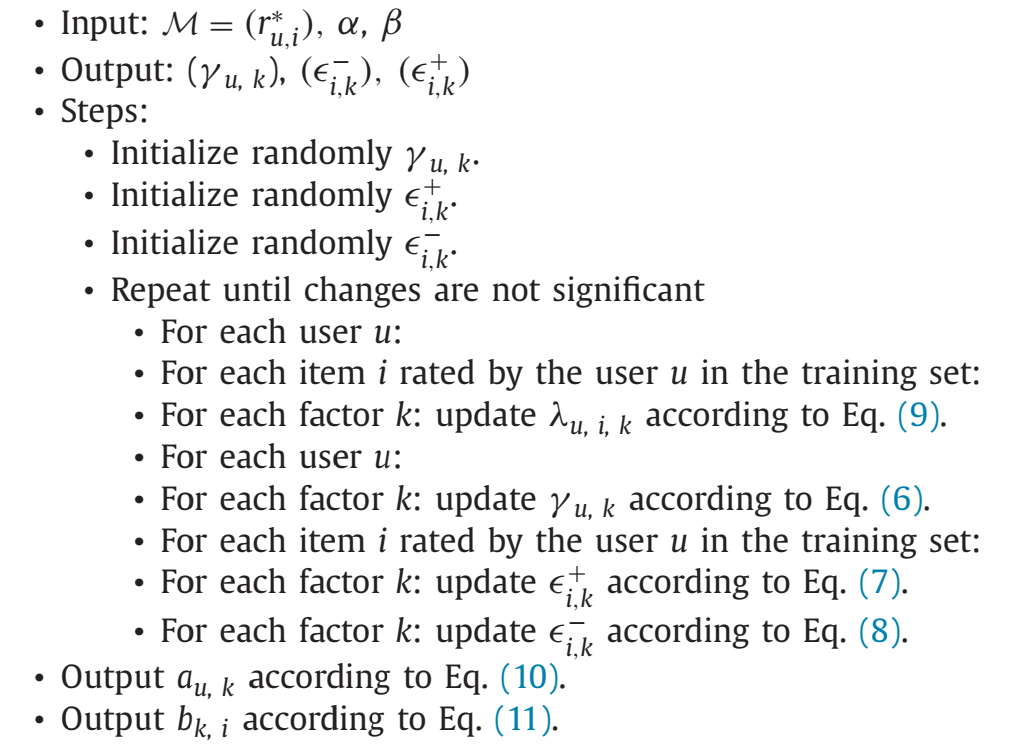
\includegraphics[width=0.7\linewidth]{fig/algorithm}
		%\caption{Example of user ratings}
		\label{fig:algorithm}
	\end{figure}
\end{frame}

\begin{frame}{Remarks}
    \begin{itemize}
        \item $ \av_{u, k}, \bv_{u, k} \in [0, 1] $, while $ \av_{u, k}, \bv_{u, k} $ can take arbitrary real values in other classical matrix factorization techinqes.
       	\item The proposed model has good probabilistic interpretations.
       	\item $K$ may be low and $\av_{u, k}, \bv_{u, k}$ are sparse.
       	\item \textbf{Proposition.} If the recommender system predicts that a user $ u $ will like the item $ i $, then there are some users with the same taste as $ u $ who have very positively rated the item $ i $.
    \end{itemize}
\end{frame}

\section{Evaluation}
\begin{frame}{Implementation}
	\begin{itemize}
		\item 실제 implementation 할 때 어떠한 방식으로 했는지? 주요하게 언급할만한 것 적기.
	\end{itemize}
\end{frame}

\begin{frame}{Evaluation}
    \begin{itemize}
        \item papaer에 나온 것처럼 영화 데이터에 대해 재현에 방점 두고 작성.
    \end{itemize}
\end{frame}

\begin{frame}{Accuracy in predictions}
    \begin{itemize}
        \item different types of errors: MAE, CMAE, 0-1-Loss 소개 및 간단히 의미 설명
        \item 각각에서 hyper parameter tuning 정해진 거 report
        \item quality of recommendations
        \item PMF(classical methods)랑 our approach 사용
        \item reproducing Table 19, 20.
    \end{itemize}
\end{frame}

\begin{frame}{Accuracy in recommendations}
    \begin{itemize}
        \item 각각에서 hyper parameter tuning 정해진 거 report
        \item quality of recommendations
        \item PMF(classical methods)랑 our approach 사용
        \item reproducing Table 19, 20.
    \end{itemize}
\end{frame}


\section{Applications}
\begin{frame}{Data description}
    \begin{itemize}
        \item 우리가 사용한 data 정리 출처 및 간단한 요약통계량
        \item 먼저 movie 로 이야기하고(논문이랑 동일), steam game and book data
    \end{itemize}
\end{frame}

\begin{frame}{Data transformation}
    \begin{itemize}
        \item steam game : transform [played time] to [rating] \\
	      for $\forall i \in \{1,2,3,4,5\},$ rating = i if \\
	      time < max ( Z(i) , Q(i) ) where Z(i) is the $20 i \%\%$ quantile of unit Gaussian, 
	      and Q(i) is the quantile of the data distribution.
	\item books : transform ratings from (0 ~ 10) to (1 ~ 5) \\
	      original [rating / 11 * 4 + 1], where [ $n$ ] is the rounded integer of $n$.
    \end{itemize}
\end{frame}

\begin{frame}{Results}
	\begin{itemize}
		\item accruacy and results of game/book applications.
		\item Game MAE : 1.1547 (PMF)
		\item Book MAE : 1.2293 (PMF)
	\end{itemize}
\end{frame}

\section{Discussion}
\begin{frame}{Discussion}
    \begin{itemize}
        \item 다양한 데이터들에 variational inference based 추천시스템을 적용해봄.
        \item 영화 이외의 domain data에 대해서도 어떤 의미가 있는지?
        \item $K$ group이 어떻게 생겼는지, 우리 직관 혹은 알려진 사실과 맞는지 확인해보는 것도 재밌을 듯.
        \item 등등 필요한 내용...
    \end{itemize}
\end{frame}

\end{document}
